\documentclass[10pt,letterpaper]{article}

\usepackage{amsmath}
\usepackage{tikz}

\newcommand{\volume}{{\ooalign{\hfil$V$\hfil\cr\kern0.08em--\hfil\cr}}}

\author{Thaddeus Hughes}
\date{\today}
\title{Adiabatic Model of a Pneumatic Cylinder}



\begin{document}
	\maketitle
	
	\begin{abstract}
		There are some basic models for pneumatic cylinders that result in modeling cylinders as constant-force devices, or nearly so. This is a rough first pass at creating a model that is a little more sophisticated. This model assumes that the air in the cylinder is adiabatic; that is, no heat transfer takes place. This model will be a differential equation intended to be used in conjunction with a numerical DE solver due to the non-linear nature of many conditions.
	\end{abstract}
	
	\section*{System Definition}
	
	We will analyze the open system that is the air contained within a pneumatic cylinder, plus the air in the hose leading up to it (inclusion of the hose will become of crucial importance and will be evident later on).
	\begin{center}
	\begin{tikzpicture}[x=1.0in,y=1.0in]
		\draw[->] (-0.5,0)--(-0.1,0) node[pos=0, left]{$P_{in}$, $\dot{\volume}_{in}$, $T_{in}$};
		
		\draw[] (0.3,-0.1)--(0,-0.1)--(0,0.1)--(0.3,0.1)--(0.3,0.5)--(1.2,0.5)--(1.2,-0.5)--(0.3,-0.5)--cycle;
		\node (state) [text width=0.4] at (0.65,0) {$m_s$ \\ $P_s$ \\ $\volume_s$ \\ $T_s$};
		\draw[->] (1.0, 0.6)--(1.4, 0.6) node[pos=0.5, above] {$v$, $x$};
		%\draw[->] (1.9,0)--(1.4,0) node[pos=0, above] {$F = P_{atm} A$};
	\end{tikzpicture}
	\end{center}
	
	Air at pressure $P_{in}$ and temperature $T_{in}$ enters the cylinder at rate $\dot{\volume}_{in}$.
	It mixes with air in the cylinder ($m_s$, $\volume_s$) and is assumed to become of uniform pressure and temperature $P_s$ and $T_s$.
	
	The piston ram is moving at velocity $v$ and with position $x$. $x$ is zero when the cylinder is bottomed out (no air in the cylinder). 
	
	\begin{center}
	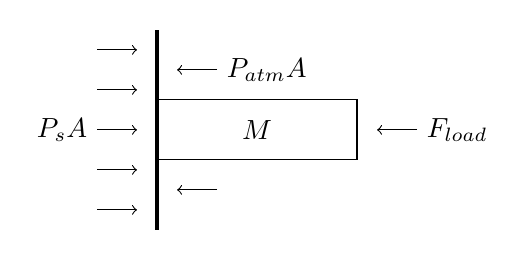
\begin{tikzpicture}[x=1.0in,y=1.0in]
		\draw[ultra thick] (0,-0.5)--(0,0.5);
		\draw[] (0,-0.15)--(0,0.15)--(1,0.15)--(1,-0.15)--cycle;
		
		\node (ctr) [] at (0.5,0) {$M$};
		
		\draw[->] (-0.3,0)--(-0.1,0) node[pos=0,left]{$P_s A$};
		\draw[->] (-0.3,0.2)--(-0.1,0.2); \draw[->] (-0.3,0.4)--(-0.1,0.4); \draw[->] (-0.3,-0.2)--(-0.1,-0.2); \draw[->] (-0.3,-0.4)--(-0.1,-0.4);
		
		\draw[->] (1.3,0)--(1.1,0) node[pos=0,right]{$F_{load}$};
		\draw[->] (0.3,0.3)--(0.1,0.3) node[pos=0,right]{$P_{atm} A$};
		\draw[->] (0.3,-0.3)--(0.1,-0.3);
	\end{tikzpicture}
	\end{center}
	
	The cylinder itself is considered to have a mass $M$ and sees the cylinder pressure, a resistive force $F_{load}$, and atmospheric pressure.
	
	\section*{Conservation Principles In The Cylinder}
	
	First, let's apply conservation of mass to the air.
	
	\begin{align}
		\frac{d}{dt} m_{sys} &= \sum_{+ in} \dot{m} \nonumber
		\\
		\frac{d}{dt} m_s &= \dot{m}_{in} \nonumber
	\end{align}
	
	We can use the ideal gas law $P \volume = m R T$ to write this in terms of knowns.
	\begin{align}
		\frac{d}{dt} m_s = \dot{m}_{in} = \frac{P_{in} \dot{\volume}_{in}}{R T_{in}}
	\end{align}
	
	Now, let's apply conservation of energy.
	
	\begin{align}
		\frac{d}{dt} E_{sys} = \sum \dot{Q}_{in} + \sum \dot{W}_{in} + \sum_{+in} \dot{m} (v^2/2 + gz + h) \nonumber
	\end{align}
	
	We will assume:
	\begin{itemize}
		\item The energy of the system is entirely thermal; $E_sys$ = $m_s u(T)$
		\item No heat transfer; $\dot{Q}_{in} = 0$
		\item Work is out of the system, defined by the pressure of the system and velocity of the ram; $\dot{W}_{in} = - \vec{F} \cdot \vec{v} = - P_s A v$
		\item Mass transfer into the system has negligible velocity ($v$) and head height ($gz$), leaving only enthalpy $h(T)$.
	\end{itemize}		
	
	\begin{align}
		\frac{d}{dt} [m_s u(T)] = - P_s A v + \dot{m}_{in} h(T_{in}) \nonumber
	\end{align}
	
	The derivative here is quite ugly, since both the mass and temperature of the system are changing. However, it can be broken up with the product rule ($\frac{d}{dt}[xy] = y \frac{dx}{dt} + x \frac{dy}{dt}$).
	
	\begin{align} 
		m_s \frac{d u(T_s)}{dt} + u(T_s) \frac{d m_s}{dt} = - P_s A v + \dot{m}_{in} h(T_{in}) \nonumber \\
		m_s \frac{d u(T_s)}{dt} = \dot{m}_{in} h(T_{in}) - P_s A v - u(T_s) \frac{d m_s}{dt} \nonumber
	\end{align}
	
	Recognizing that $u(T)$ and $h(T)$ can be approximated as $u(T) = c_p T$ and $h(T) = c_v T$, we can then solve the equation for $\frac{dT_s}{dt}$.
	
	\begin{align} 
		\frac{d T_s}{dt} = \frac{ \dot{m}_{in} c_v T_{in} - P_s A v - c_p T_s \dot{m}_{in} }{c_p m_s}
	\end{align}
	
	All of these are knowns or states aside from $P_s$, which can be determined with the ideal gas law, and the modeling of the system volume as based on cylinder extension, crossectional area, and initial (i.e. hose) dead volume.
	
	\begin{align}
		P_s = \frac{m_s R T_s}{\volume_s} \nonumber \\
		P_s = \frac{m_s R T_s}{\volume_{dead} + x A}
	\end{align}
	
	\section*{Conservation Principles on the Piston}
	
	We can simply apply conservation of linear momentum to the piston.
	
	\begin{align}
		\frac{d}{dt} P_{sys}= \sum F + \sum \dot{m} v \nonumber
	\end{align}
	
	We will assume:
	\begin{itemize}
		\item No mass transfer in this system, so $\frac{d}{dt} P_{sys} = M \frac{dv}{dt}$ and $\dot{m}=0$
		\item The forces acting on the piston are the cylinder pressure, atmospheric pressure, and the external load.
	\end{itemize}
	
	\begin{align}
		M \frac{dv}{dt} &= P_s A - P_{atm} A - F_{load} \nonumber \\
		\frac{dv}{dt} &= \frac{(P_s - P_{atm}) A - F_{load}}{M}
	\end{align}
	
	We are also interested in the position of the piston.
	
	\begin{align}
		\frac{dx}{dt} = v
	\end{align}
	
	\section*{Limiting the Model}
	In review we have:
	
	\begin{itemize}
		\item A model for rate of change of $m_s$
		\item A model for rate of change of $T_s$
		\item Supporting equation for cylinder pressure $P_s$
		\item A model for velocity $v$
		\item A model for position $x$
	\end{itemize}
	
	We simply now need initial conditions, "bumper" conditions, and termination criteria.
	
	We will assume the initial temperature $T_s$ will be set to that of the input gas $T_{in}$. (This may seem like it would negate all the point of this model, but recall that when gases expand/contract, they change pressure)
	
	\begin{align}
		T_s(t=0) = T_{in}
	\end{align}
	
	The initial mass of cylinder air can be found with the ideal gas law, assuming we start at atmospheric pressure (wholly unpressurized)
	
	\begin{align}
		m_s(t=0 = \frac{P_{atm} \volume_{dead}}{R T_s(t=0)}
	\end{align}
	
	There's an interesting edge case that our model doesn't look at, and that's when we overfill the cylinder. It's not reas
	
	Assume the piston starts from rest.
	
	\begin{align}
		x(t=0) &= 0 \\
		v(t=0) &= 0
	\end{align}
		
	
\end{document}